\chapter{Diagramma dei casi d'uso}

\section{Registrazione}
\begin{figure}[h!]
\centering
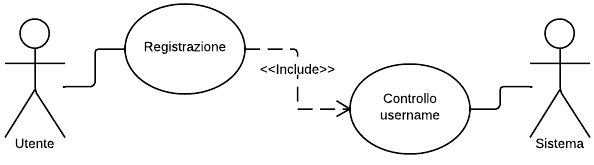
\includegraphics[scale=0.60]{img/use/Reg.png}
\caption{Registrazione}
\label{fig:registrazione}
\end{figure}
\begin{table}[H]
\begin{tabular}{p{0.35\textwidth}|p{0.65\textwidth}}
\toprule
NOME & Registrazione;\\
\hline
OBBIETTIVO: & Registrare l utente nella applicazione;\\
\hline
PRE-CONDIZIONE & L'utente non deve essere registrato nel sistema;\\
\hline
SUCCESSO: & La registrazione avviene con successo;\\
\hline
FALLIMENTO: & Non è possibile effettuare la registrazione; \\
\hline
ATTORE PRIMARIO: & Utente;\\
\hline
ATTORI SECONDARI: & Sistema;\\
\bottomrule
\end{tabular}
\caption{Registrazione Utente}
\label{table:reg}
\end{table}
FLUSSO PRINCIPALE:
\begin{enumerate}
\item L'utente compila e inoltra il modulo d'iscrizione;
\begin{enumerate}
\item Controllo dei campi non opzionali e necessari alla registrazione;
\item Doppio inserimento password;
\end{enumerate}
\item Controllo del username;
\item Ricerca del username;
\begin{enumerate}
\item Il sistema verifica che l'utente (username univoco) non sia già registrato;
\end{enumerate}
\item Avviene la registrazione del utente;
\item La registrazione è avvenuta con successo;
\end{enumerate}

\section{Login}
\begin{figure}[h!]
\centering
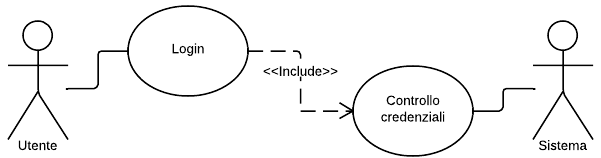
\includegraphics[scale=0.50]{img/use/Log.png}
\caption{Login}
\label{fig:Login}
\end{figure}
\begin{table}[H]
\begin{tabular}{p{0.35\textwidth}|p{0.65\textwidth}}
\toprule
NOME & Login;\\
\hline
OBBIETTIVO: & Ottenere accesso all'applicazione;\\
\hline
PRE-CONDIZIONE & L'utente deve essere registrato all'applicazione;\\
\hline
SUCCESSO: & L'utente ottiene accesso all'applicazione;\\
\hline
FALLIMENTO: & La procedura non va a buon fine;\\
\hline
ATTORE PRIMARIO: & Utente;\\
\hline
ATTORI SECONDARI: & Sistema;\\
\bottomrule
\end{tabular}
\caption{Login Utente}
\label{table:log}
\end{table}
FLUSSO PRINCIPALE:
\begin{enumerate}
\item L'utente immette le proprie credenziali;
\item L'utente inoltra la richiesta di accesso;
\begin{enumerate}
\item Il sistema verifica la corrispondenza delle credenziali;
\end{enumerate}
\item L'utente ottiene accesso al' applicazione;
\end{enumerate}

\section{Crea Evento}
\begin{figure}[h!]
\centering
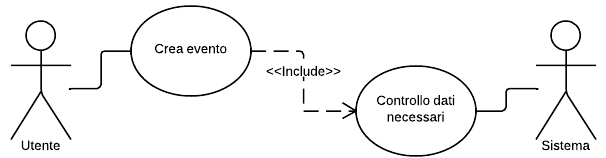
\includegraphics[scale=0.60]{img/use/creaevento.png}
\caption{Crea evento}
\label{fig:creaeve}
\end{figure}
\begin{table}[H]
\begin{tabular}{p{0.35\textwidth}|p{0.65\textwidth}}
\toprule
NOME & Crea evento;\\
\hline
OBBIETTIVO: & Creare un evento;\\
\hline
PRE-CONDIZIONE & L'utente deve essere registrato all'applicazione;
L'utente deve aver eseguito l'accesso all'applicazione;\\
\hline
SUCCESSO: & L'utente crea l'evento;\\
\hline
FALLIMENTO: & La procedura non va a buon fine;\\
\hline
ATTORE PRIMARIO: & Utente;\\
\hline
ATTORI SECONDARI: & Sistema;\\
\bottomrule
\end{tabular}
\caption{Crea evento}
\label{table:creaevento}
\end{table}
FLUSSO PRINCIPALE:
\begin{enumerate}
\item L'utente immette i dati necessari alla creazione dell'evento;
\item L'utente inoltra la richiesta di creazione;
\begin{enumerate}
\item Il sistema verifica i dati inseriti;
\end{enumerate}
\item L'utente ha creato l'evento;
\end{enumerate}

\section{Partecipazione ad evento – Utente senza accesso}
\begin{figure}[h!]
\centering
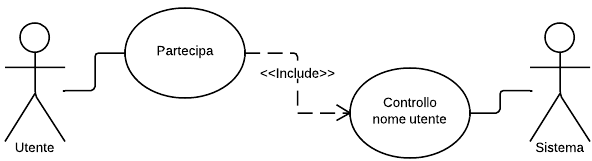
\includegraphics[scale=0.60]{img/use/PartecipaSa.png}
\caption{Partecipazione senza accesso}
\label{fig:ParteSA}
\end{figure}

\begin{table}[H]
\begin{tabular}{p{0.35\textwidth}|p{0.65\textwidth}}
\toprule
NOME & Partecipazione ad evento senza accesso;\\
\hline
OBBIETTIVO: & L'utente rende la propria disponibilità per un evento senza essere registrato all'applicazione;\\
\hline
PRE-CONDIZIONE & Nessuna;\\
\hline
SUCCESSO: & L'utente si rende disponibile per tale evento;\\
	\hline
FALLIMENTO: & La procedura non va a buon fine;\\
\hline
ATTORE PRIMARIO: & Utente;\\
\hline
ATTORI SECONDARI: & Sistema;\\
\bottomrule
\end{tabular}
\caption{Partecipazione ad evento senza accesso}
\label{table:parSA}
\end{table}
FLUSSO PRINCIPALE:
\begin{enumerate}
\item L'utente seleziona l'evento desiderato e visualizza tutte le informazioni riguardanti l'evento;
\begin{enumerate}
\item L'utente visualizza la lista di tutti gli utenti iscritti all'evento e il username dell'utente che l ha creato;
\item L'utente visualizza la lista di tutti i commenti per l evento selezionato;
\end{enumerate}
\item L'utente inserisce il proprio nome nel apposito spazio;
\begin{enumerate}
\item Il sistema verifica che l'utente ha inserito correttamente il suo nome;
\end{enumerate}
\item L'utente inoltra la richiesta d iscrizione;
\item L'Utente si rende disponibile per tale evento;
\end{enumerate}

\section{Partecipazione ad evento – Utente con accesso}
\begin{figure}[h!]
\centering
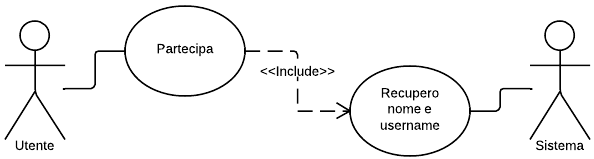
\includegraphics[scale=0.60]{img/use/PartecipaCa.png}
\caption{Partecipazione con accesso}
\label{fig:ParteCA}
\end{figure}
\begin{table}[H]
\begin{tabular}{p{0.35\textwidth}|p{0.65\textwidth}}
\toprule
NOME & Partecipazione ad evento con accesso;\\
\hline
OBBIETTIVO: & L'utente rende la propria disponibilità per un evento dopo aver eseguito l'accesso all'applicazione;\\
\hline
PRE-CONDIZIONE & L'utente deve essere registrato all'applicazione;\\
\hline
SUCCESSO: & L'utente si rende disponibile per tale evento;\\
\hline
FALLIMENTO: & La procedura non va a buon fine;\\
\hline
ATTORE PRIMARIO: & Utente;\\
\hline
ATTORI SECONDARI: & Sistema;\\
\bottomrule
\end{tabular}
\caption{Partecipazione ad evento con accesso}
\label{table:par2}
\end{table}
FLUSSO PRINCIPALE:
\begin{enumerate}
\item L'utente seleziona l'evento desiderato e visualizza tutte le informazioni riguardanti l'evento;
\begin{enumerate}
\item L'utente visualizza la lista di tutti gli utenti iscritti all'evento e il username dell'utente che l ha creato;
\item L'Utente visualizza la lista di tutti i commenti per l evento selezionato;
\end{enumerate}
\item L'utente inoltra la richiesta d iscrizione;
\begin{enumerate}
\item Il Sistema recupera il nome del utente che ha eseguito l accesso;
\item Il Sistema recupera il username del utente che ha eseguito l accesso;
\end{enumerate}
\item L'utente si rende disponibile per tale evento;
\begin{enumerate}
\item L'utente può lasciare commenti per l evento selezionato;
\end{enumerate}
\end{enumerate}

\section{Chiudere evento}
\begin{figure}[H]
\centering
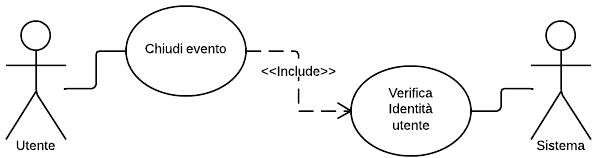
\includegraphics[scale=0.60]{img/use/Chiude.png}
\caption{Chiudere un evento}
\label{fig:Chiudere}
\end{figure}
\begin{table}[H]
\begin{tabular}{p{0.35\textwidth}|p{0.65\textwidth}}
\toprule
NOME & Chiusura di un evento;\\
\hline
OBBIETTIVO: & L utente chiude un evento;\\
\hline
PRE-CONDIZIONE & L'utente deve essere registrato all'applicazione;
L'utente è il creatore dell'evento;\\
\hline
SUCCESSO: & L utente chiude correttamente l evento;\\
\hline
FALLIMENTO: & La procedura non va a buon fine;\\
\hline
ATTORE PRIMARIO: & Utente;\\
\hline
ATTORI SECONDARI: & Sistema;\\
\bottomrule
\end{tabular}
\caption{Chiudere un evento}
\label{table:chiude}
\end{table}	
FLUSSO PRINCIPALE:
\begin{enumerate}
\item L'utente seleziona l'evento desiderato;
\item L'utente inserisce le eventuali cause che hanno portato alla chiusura dell'evento;
\item L'utente inoltra la richiesta di chiusura dell'evento;
\begin{enumerate}
\item Il Sistema controlla che l'utente che vuole chiudere l evento sia il creatore dello stesso;
\end{enumerate}
\item L utente ha chiuso l'evento;
\end{enumerate}

\section{Eliminazione evento}
\begin{figure}[H]
\centering
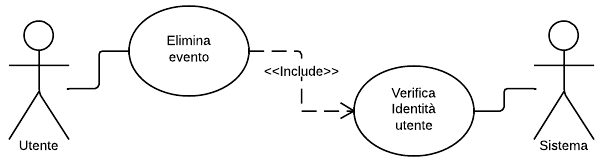
\includegraphics[scale=0.60]{img/use/Elimina.png}
\caption{Eliminare un evento}
\label{fig:Elimina}
\end{figure}
\begin{table}[H]
\begin{tabular}{p{0.35\textwidth}|p{0.65\textwidth}}
\toprule
NOME & Eliminazione di un evento;\\
\hline
OBBIETTIVO: & L'utente elimina un evento;\\
\hline
PRE-CONDIZIONE & L'utente deve essere registrato all'applicazione;
L'utente è il creatore dell'evento;\\
\hline
SUCCESSO: & L utente elimina correttamente l evento;\\
\hline
FALLIMENTO: & La procedura non va a buon fine;\\
\hline
ATTORE PRIMARIO: & Utente;\\
\hline
ATTORI SECONDARI: & Sistema;\\
\bottomrule
\end{tabular}
\caption{Eliminare di un evento}
\label{table:elimina}
\end{table}	
FLUSSO PRINCIPALE:
\begin{enumerate}
\item L'utente seleziona l'evento desiderato;
\item L'utente inoltra la richiesta di eliminazione dell'evento;
\begin{enumerate}
\item Il sistema controlla che l'utente che vuole eliminare l evento sia il creatore dello stesso;
\end{enumerate}
\item L'utente ha eliminato l'evento;
\end{enumerate}

\section{Diagramma casi d'uso completo}
\begin{figure}[H]
\centering
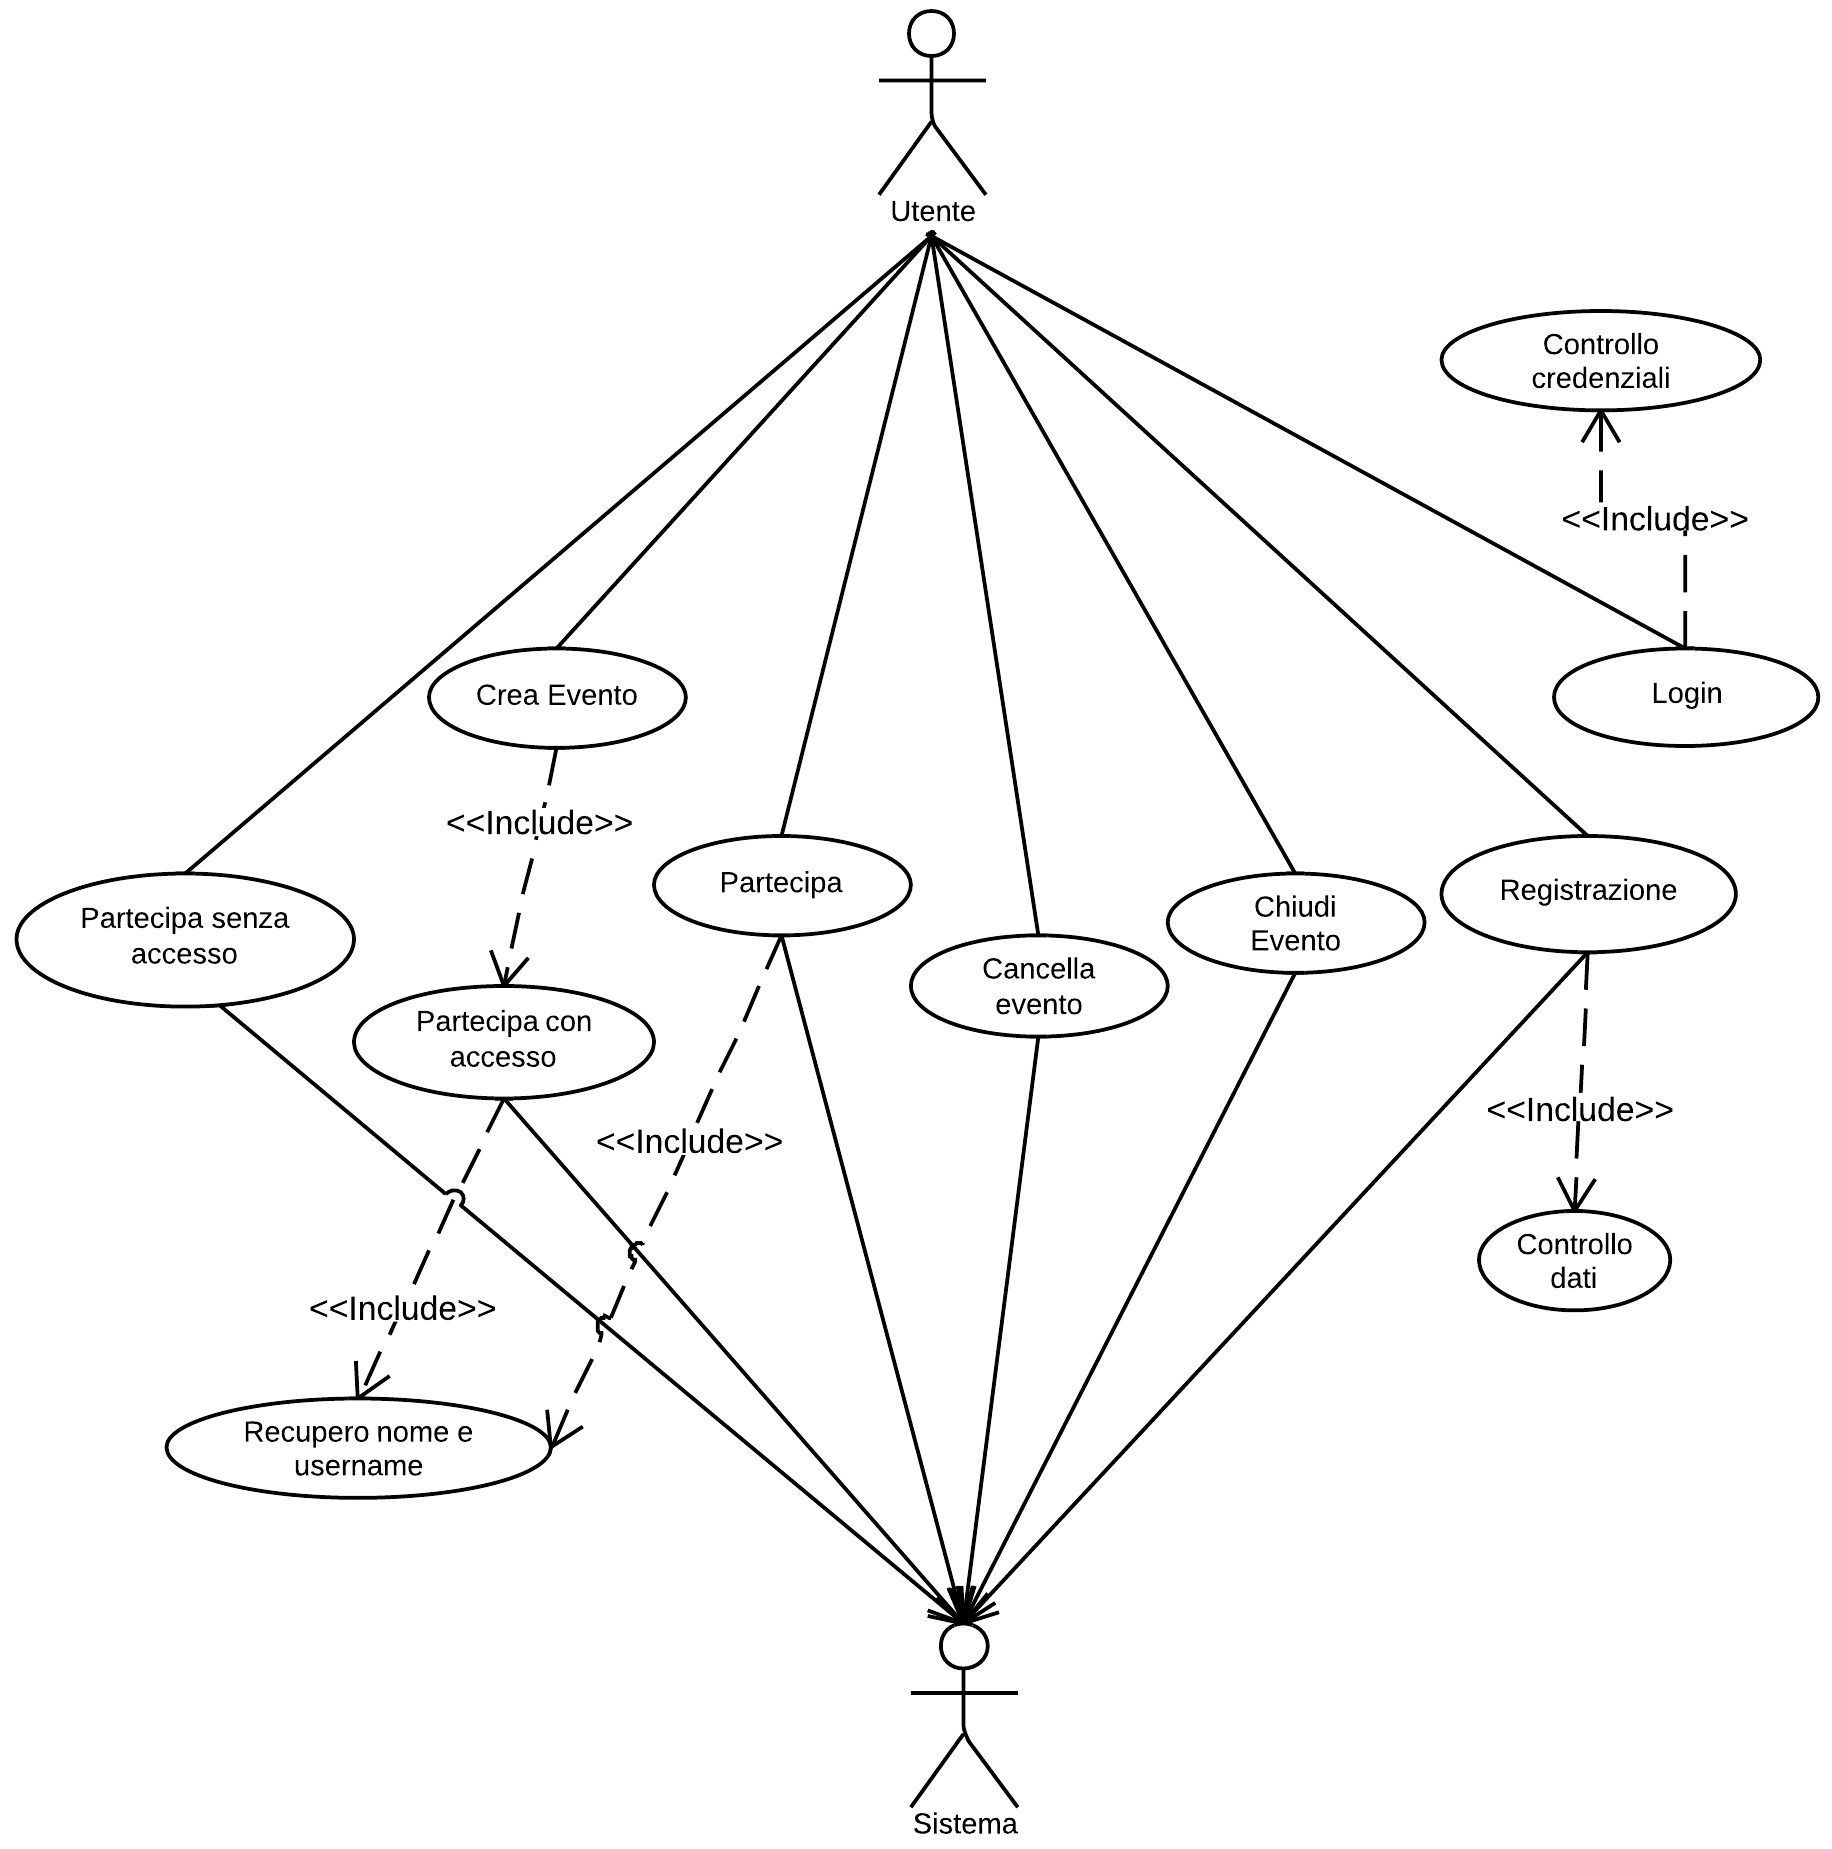
\includegraphics[width=16cm, height=14cm]{img/use/DiagUsocompleto.png}
\caption{Diagramma casi d'uso}
\label{fig:diagcompl}
\end{figure}



